\documentclass{beamer}

% Top-aligning columns within a top-aligned frame
% https://tex.stackexchange.com/questions/16447/beamer-top-aligning-columns-within-a-top-aligned-frame
\makeatletter
\newenvironment{myitemize}{%
   \setlength{\topsep}{0pt}
   \setlength{\partopsep}{0pt}
   \renewcommand*{\@listi}{\leftmargin\leftmargini \parsep\z@ \topsep\z@ \itemsep\z@}
   \let\@listI\@listi
   \itemize
}{\enditemize}
\makeatother  

\usepackage[USenglish]{babel}
\usepackage[utf8]{inputenc}
\usepackage{amssymb, amsmath}
\usepackage{bm}
\usepackage{color}
\usepackage{tikz}
\usepackage{url}

\definecolor{links}{HTML}{2A1B81}
\hypersetup{colorlinks,linkcolor=,urlcolor=links}

\usetheme{Boadilla}
\setbeamertemplate{headline}{}
\newcommand*\oldmacro{}%
\let\oldmacro\insertshorttitle%
\renewcommand*\insertshorttitle{%
  \oldmacro\hfill%
  \insertframenumber\,/\,\inserttotalframenumber}
  

\bibliographystyle{apalike}
% make bibliography entries smaller
%\renewcommand\bibfont{\scriptsize}
% Now get rid of all the colours
\setbeamercolor*{bibliography entry title}{fg=black}
\setbeamercolor*{bibliography entry author}{fg=black}
\setbeamercolor*{bibliography entry location}{fg=black}
\setbeamercolor*{bibliography entry note}{fg=black}

% and kill the abominable icon
\setbeamertemplate{bibliography item}{}

\begin{document}
\title{Adversarial Network Compression}  
\author{Radek Bartyzal}
\date{\today} 
\institute{Let's talk ML in Prague}

\frame{\titlepage} 

\begin{frame}{Prior work}


\begin{block}{Ensembles}
Diverse models with similar validation performances can be often be combined to achieve predictive
power superior to each of the constituent models. \cite{cit:ensembles}
\end{block}

\begin{block}{Born again trees}
Learn a single tree that is able to recover the performance of a multiple-tree predictor. \cite{cit:bat}
\end{block}

\begin{block}{Knowledge distillation = model compression}
Transfer knowledge acquired by a learned
teacher model to a new simpler student model. \cite{cit:distill}
\end{block}



\end{frame}
%--------- END Frame 1 -------------

\begin{frame}[t]{Knowledge distillation}

\begin{columns}[t]
\begin{column}{0.5\textwidth}
Teacher
\begin{itemize}
\item high-capacity model
\item good performance
\end{itemize}
\end{column}

\begin{column}{0.5\textwidth}
Student
\begin{itemize}
\item more compact model
\item not as good performance as the teacher but better than if it was trained without it
\end{itemize}
\end{column}

\end{columns}

\vfill
By transferring knowledge, one hopes to benefit from the student’s
compactness while suffering only minimal degradation in performance.

\end{frame}
%--------- END Frame 2 -------------

\begin{frame}{Knowledge distillation}

Teacher produces soft targets = probabilities of incorrect classes = the key to generalization outside of the training dataset.

\vfill

Training student = minimize weighted average of:

\begin{itemize}
\item cross entropy with the soft targets
\item cross entropy with the hard targets = labels
\end{itemize}


\end{frame}
%--------- END Frame 3 -------------

\begin{frame}{Knowledge distillation results}

\begin{figure}[h]
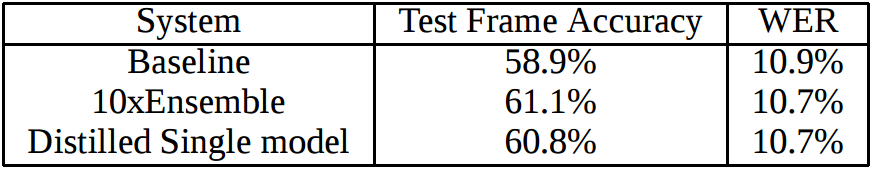
\includegraphics[width=\textwidth]{img/distilled_result}
\caption{DNN acoustic models used in Automatic Speech Recognition. Distilled model trained by an ensemble of models performs better than the baseline. \cite{cit:distill}}
\end{figure}

\end{frame}
%--------- END Frame 4 -------------
\begin{frame}{Generative Adversarial Networks}

\begin{itemize}
\item Generator G tries to create images that look real = approximate train data distribution
\item Discriminator D tries to distinguish real images from G's images
\end{itemize}

\begin{figure}[h]
\includegraphics[width=\textwidth]{img/cGAN}
\end{figure}

\end{frame}
%--------- END Frame 4 -------------
\begin{frame}{Adversarial Network Compression}

\begin{itemize}
\item teacher is trained on hard labels and then frozen
\item student trained only on soft targets = no labels
\item teacher and student have the same architecture
\item architectures are CNN ResNets
\item using GAN discriminator to align the teacher-student distributions
\item last layer (before logits) features are given to discriminator
\item L2 loss of logits from student VS teacher forces student to mimic teacher 
\end{itemize}

\begin{block}{Logits}
Unscaled log-probability values = before the softmax
activation function.
\end{block}


\end{frame}
%--------- END Frame 5 -------------
\begin{frame}{Adversarial Network Compression}

\begin{figure}[h]
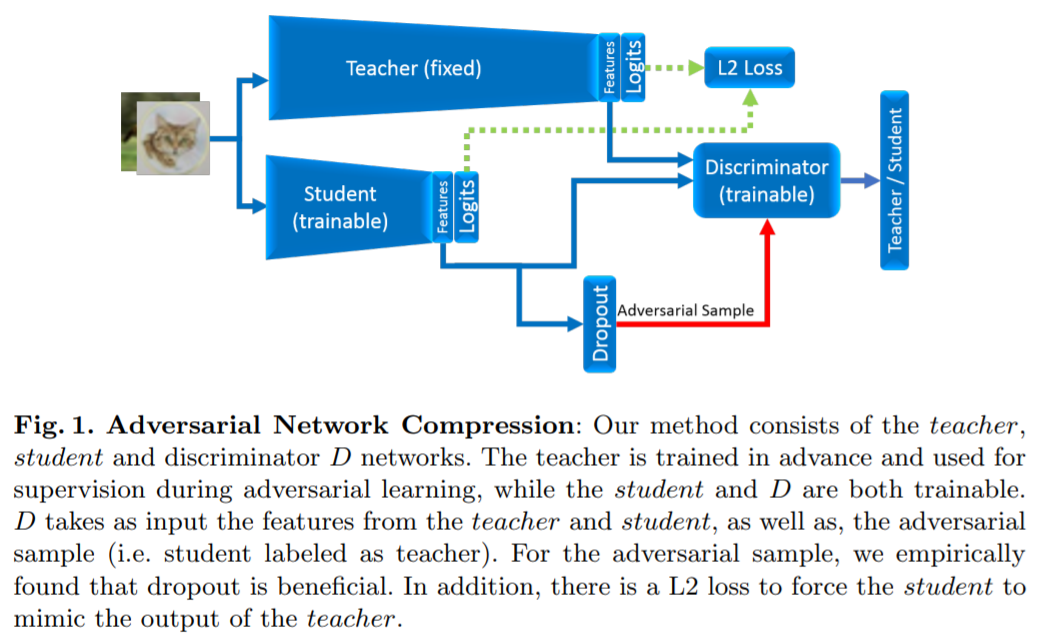
\includegraphics[width=\textwidth]{img/GAN_distill}
\end{figure}

\end{frame}
%--------- END Frame 6 -------------

%--------- END Frame 7 -------------
\begin{frame}{Adversarial Network Compression}




\end{frame}
%--------- END Frame 6 -------------
\begin{frame}{Residual Networks (ResNet)}
\begin{itemize}
\item Add skip-connection that bypasses the non-linear transformations with an identity function.
\item Identity function and the output of previous layer are combined by summation, which may impede the information flow in the network.
\item "Thin and deep" = small number of filters, 1000+ layers
\end{itemize}

\begin{block}{Diminishing feature reuse}
Gradient flowing through skip connections is not forced to go through residual block weights $\implies$ 

\begin{itemize}
\item few blocks learn useful representations 
\item many blocks share very little information with
small contribution to the final goal
\end{itemize}
\end{block}

\end{frame}
%--------- END Frame 9 -------------
\begin{frame}{ResNet: Residual block}
\begin{figure}[h]
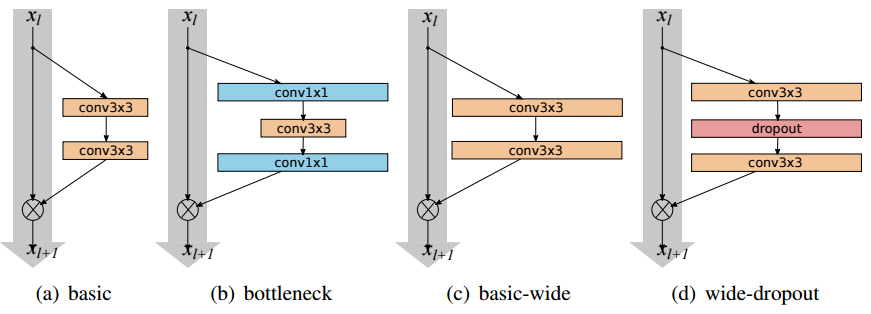
\includegraphics[width=\textwidth]{img/resnet_blocks}
\caption{Various residual blocks used in the paper. Batch normalization and ReLU precede
each convolution (omitted for clarity). \cite{cit:resnet}}
\end{figure}
\end{frame}



%--------- END Frame 12 -------------
\begin{frame}{Sources}

\begin{thebibliography}{0}

  \bibitem[1]{cit:ban} 1. Belagiannis, Vasileios, Azade Farshad, and Fabio Galasso. "Adversarial Network Compression." arXiv preprint arXiv:1803.10750 (2018). Accessible from: \url{https://arxiv.org/abs/1803.10750}
  
  \bibitem[2]{cit:stat} 2. Breiman, Leo. "Statistical modeling: The two cultures (with comments and a rejoinder by the author)." Statistical science 16.3 (2001): 199-231. Accessible from: \url{https://projecteuclid.org/download/pdf_1/euclid.ss/1009213726\%20}
  
  \bibitem[3]{cit:ensembles} 3. Hansen, Lars Kai, and Peter Salamon. "Neural network ensembles." IEEE transactions on pattern analysis and machine intelligence 12.10 (1990): 993-1001.
\end{thebibliography}

\end{frame}


\begin{frame}{Sources}

\begin{thebibliography}{0}
  \bibitem[4]{cit:bat} 4. Breiman, Leo, and Nong Shang. "Born again trees." ps (1996). Accessible from: \url{https://www.stat.berkeley.edu/~breiman/BAtrees.pdf}
  
  \bibitem[5]{cit:distill} 5. Hinton, Geoffrey, Oriol Vinyals, and Jeff Dean. "Distilling the knowledge in a neural network." arXiv preprint arXiv:1503.02531 (2015). Accessible from: \url{https://arxiv.org/pdf/1503.02531.pdf}
  

\end{thebibliography}

\end{frame}
 
 
 
\end{document}
